
\documentclass{article}

\usepackage{tikz,times}
\usepackage[paperwidth=25cm,paperheight=22cm,left=1cm,top=1cm]{geometry}

\usetikzlibrary{mindmap,backgrounds}

\pagestyle{empty}

\begin{document}

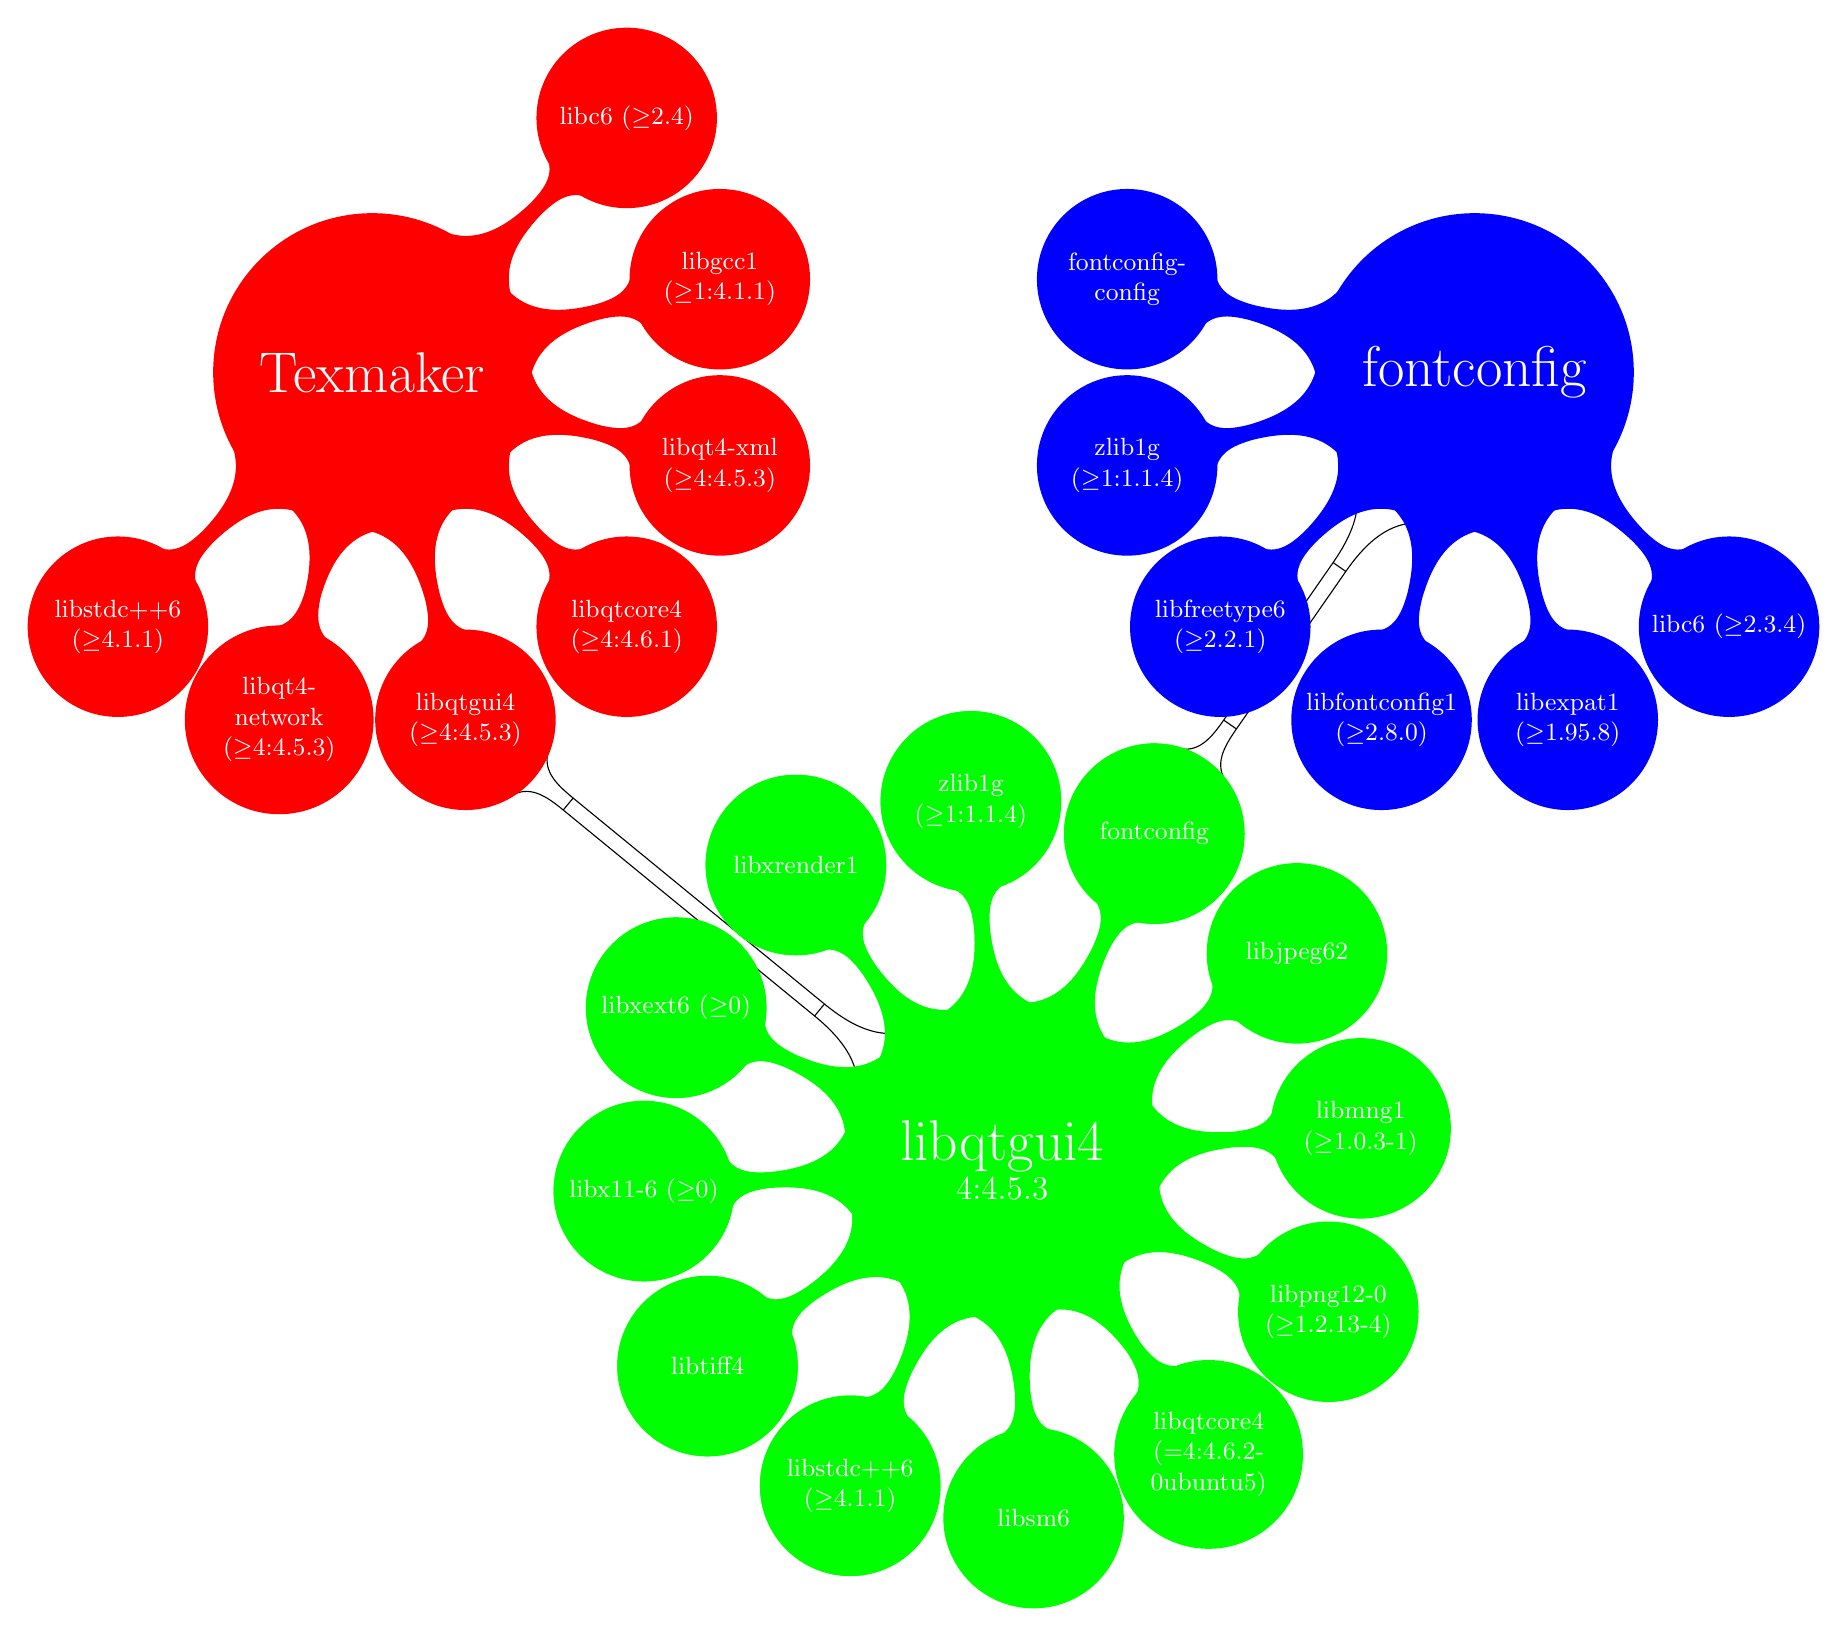
\begin{tikzpicture}[mindmap,
  level 1 concept/.append style={level distance=130,sibling angle=30},
  extra concept/.append style={color=blue!50,text=black}]

  % Applied area: computer science and its subfields

 % \begin{scope}[mindmap, concept color=orange, text=white]
 %   \node [concept] at (-5,10) (kernel) {\huge Noyau}[clockwise from=-5] 
 %     child {node [concept] (dots) {...}}
 %     child {node [concept] (proc) {Processus}}
 %     child {node [concept] (res) {R{\'e}seaux}}
 %     child {node [concept] (usb) {USB}}
 %     child {node [concept] (key) {Clavier \& Souris}}
 %     child {node [concept] (aff) {Affichage}}
 %     child {node [concept] (file) {Fichiers}};
 % \end{scope}

  % Applied area: theoretical physics and its subfields

  \begin{scope}[mindmap, concept color=red,text=white]
    \node [concept] at (-5,0) (tex) {\huge Texmaker}[clockwise from=45] 
      child% [level distance=160]
        {node [concept] (libc) {libc6 ($\geq$2.4)}}
      child {node [concept] (libgcc) {libgcc1 ($\geq$1:4.1.1)}}
      child {node [concept] (qt4) {libqt4-xml ($\geq$4:4.5.3)}}
      child {node [concept] (qtcore) {libqtcore4 ($\geq$4:4.6.1)}}
      child {node [concept] (qtgui4) {libqtgui4 ($\geq$4:4.5.3)}}
      child {node [concept] (net) {libqt4-network ($\geq$4:4.5.3)}}
      child {node [concept] (stdc) {libstdc++6 ($\geq$4.1.1)}};
  \end{scope}
  
  
   \begin{scope}[mindmap, concept color=green,text=white]
    \node [concept] at (+3,-10) (gui4) {{\huge libqtgui4} 4:4.5.3}[clockwise from=-115] 
      child {node [concept] {libaudio2}}
      child {node [concept] {libc6 ($\geq$2.11)}}
      child {node [concept] {libfontconfig1 ($\geq$2.8.0)}}
      child {node [concept] {libfreetype6 ($\geq$2.3.5)}}
      child {node [concept] {libgcc1 ($\geq$1:4.1.1)}}
      child {node [concept] {libglib2.0-0 ($\geq$2.12.0)}}
      child {node [concept] {libice6 ($\geq$1:1.0.0)}}
      child {node [concept] {libjpeg62}}
      child {node [concept] {libmng1 ($\geq$1.0.3-1)}}
      child {node [concept] {libpng12-0 ($\geq$1.2.13-4)}}
      child {node [concept] {libqtcore4 (=4:4.6.2-0ubuntu5)}}
      child {node [concept] {libsm6}}
      child {node [concept] {libstdc++6 ($\geq$4.1.1)}}
      child {node [concept] {libtiff4}}
      child {node [concept] {libx11-6 ($\geq$0)}}
      child {node [concept] {libxext6 ($\geq$0)}}
      child {node [concept] {libxrender1}}
      child {node [concept] {zlib1g ($\geq$1:1.1.4)}}
      child {node [concept] (lfont) {fontconfig}};
  \end{scope}
  

\begin{scope}[mindmap, concept color=blue,text=white]
    \node [concept] at (+9,0) (font) {{\huge fontconfig}}[clockwise from=-45] 
      child {node [concept] {libc6 ($\geq$2.3.4)}}
      child {node [concept] {libexpat1 ($\geq$1.95.8)}}
      child {node [concept] {libfontconfig1 ($\geq$2.8.0)}}
      child {node [concept] {libfreetype6 ($\geq$2.2.1)}}
      child {node [concept] {zlib1g ($\geq$1:1.1.4)}}
      child {node [concept] {fontconfig-config}};
  \end{scope}
  
  
 \begin{pgfonlayer}{background}
    \draw [circle connection bar]
      (qtgui4) edge (gui4)
      (lfont) edge (font);
  \end{pgfonlayer}
  
\end{tikzpicture}

\end{document}
